% Section content template for individual Educative lessons
% This file contains the actual content for a specific section
% Generated from Educative API section content

% Section: SOLID: Open Closed Principle
% Section ID: 6348852334690304
% Section Slug: solid-open-closed-principle
% Generated: 2025-12-11T05:50:09.784518

\subsection{Introduction}\label{introduction}
\\
In 1988, Bertrand Meyer defined the \textbf{Open Closed Principle (OCP)} in the following way, ``A software artifact should be open for extension but closed for modification.'' This means that a system should improve easily by adding new code instead of changing the code core. This way, the core code always retains its unique identity, making it reusable.
\\
One might think of OCP as inheritance, but remember that inheritance is only one of the OCP techniques. We use the interface because it is open for extension and closed for modification. Therefore, OCP is also defined as \textbf{polymorphic OCP.}

\subsection{Example}\label{YtqjB_wrWdYqOi9OqVU-g}
\\
Suppose Alex had a cardboard business that sold boxes to its clients. We designed a class for calculating the volume of boxes. It takes the dimensions and calculates the volume of each box and adds it up to calculate the total volume of all boxes, as shown below.

\begin{figure}[htbp]
 \centering
 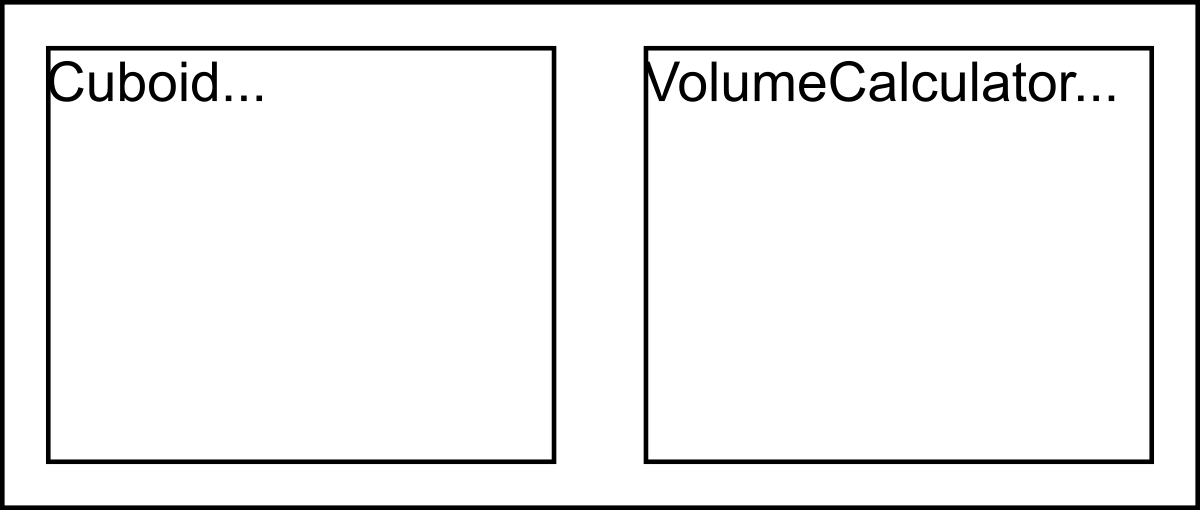
\includegraphics[width=0.5\textwidth]{Images/chapter_4/section_6348852334690304/4564738661154816.png}
 \caption{The volume calculator class}
\end{figure}

The algorithm for the \texttt{volume(Cuboid)} function is shown in the flowchart below.

\begin{figure}[htbp]
 \centering
 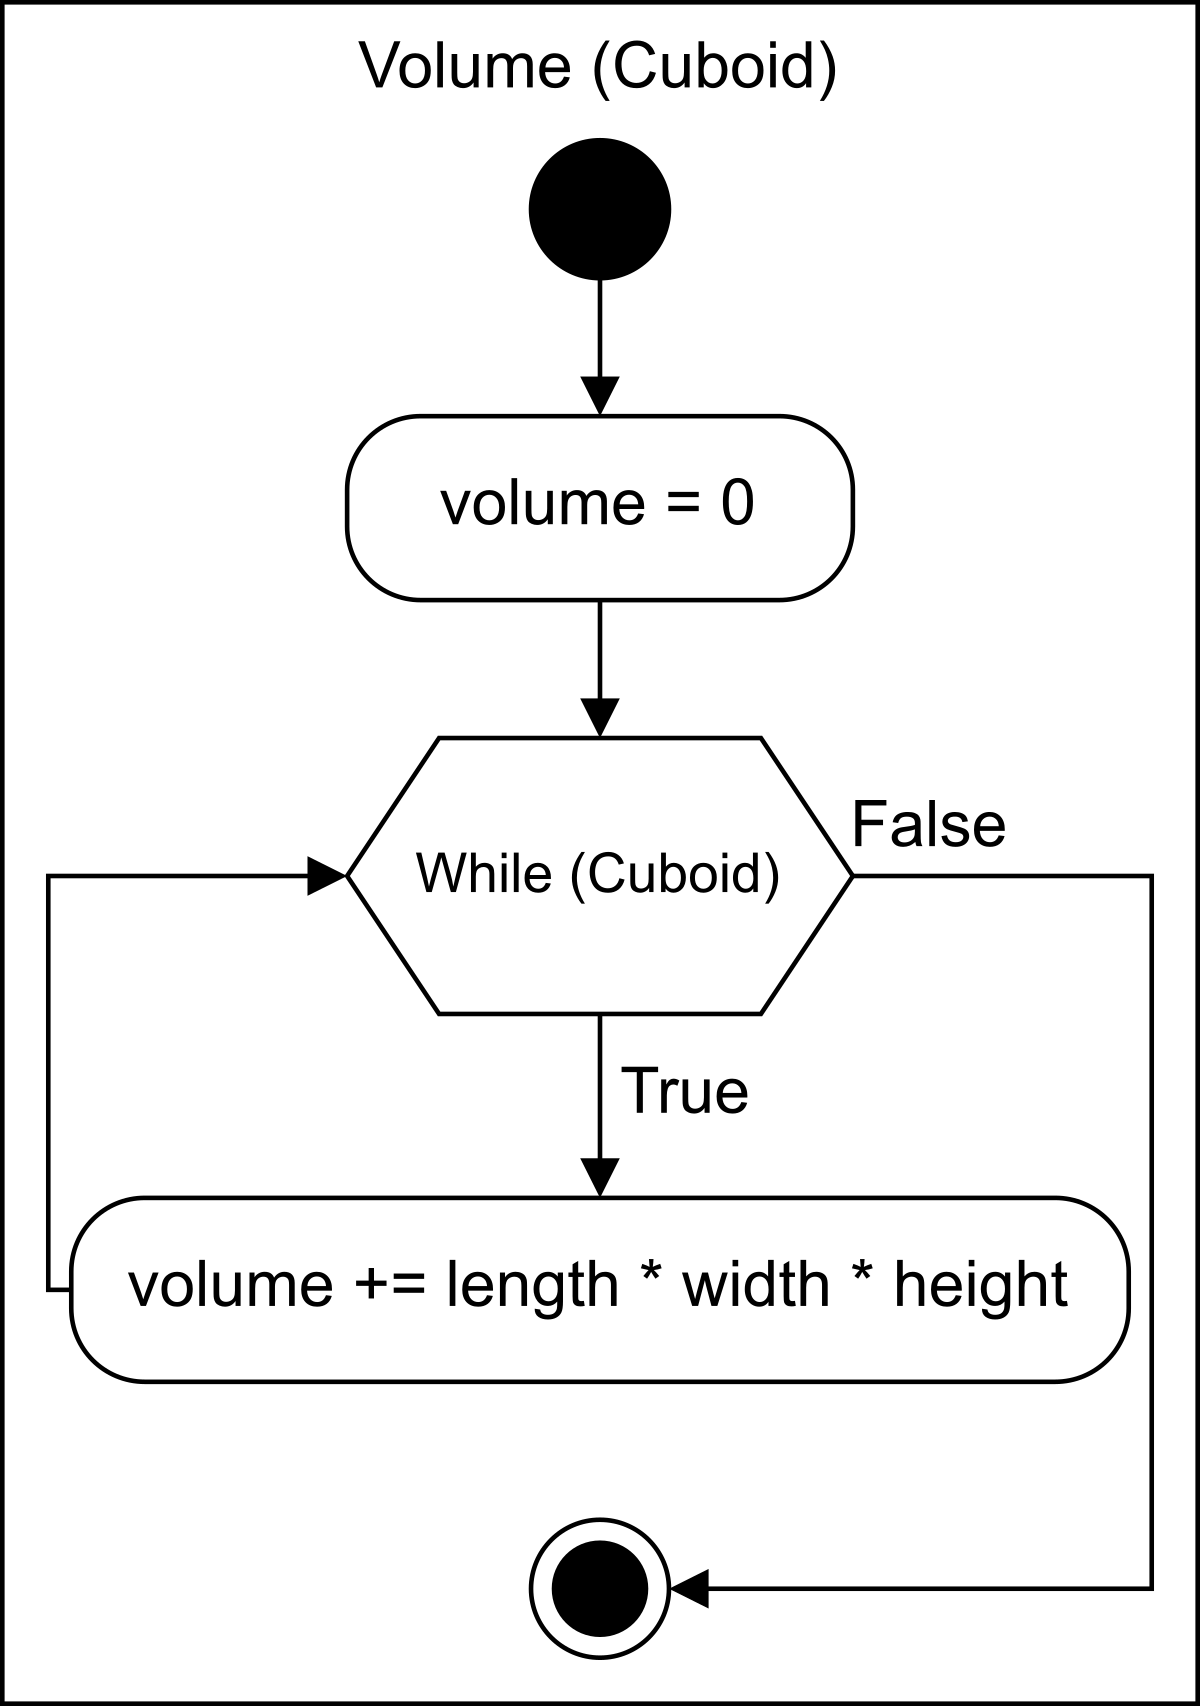
\includegraphics[width=0.25\textwidth]{Images/chapter_4/section_6348852334690304/5064238654816256.png}
 \caption{The volume(Cuboid) function}
\end{figure}

As the business grew, Alex also started selling cone-shaped boxes. To integrate the calculation of its volume, we need to make a \texttt{Cone} class and update the \texttt{volume()} function. See the updated classes below:

\begin{figure}[htbp]
 \centering
 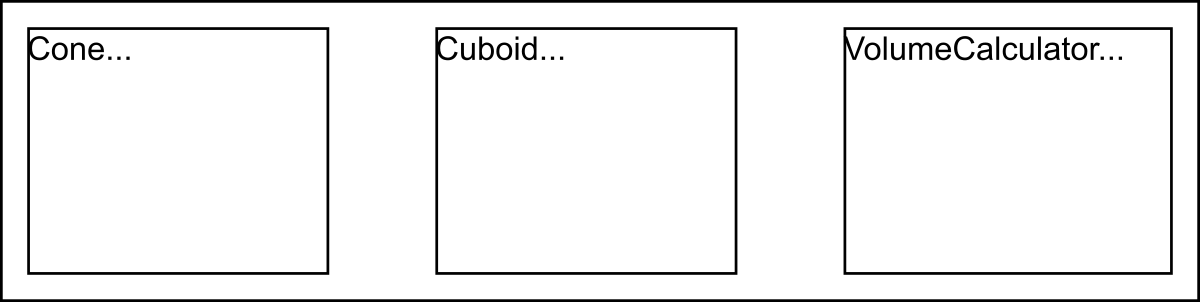
\includegraphics[width=0.5\textwidth]{Images/chapter_4/section_6348852334690304/5264251322368000.png}
 \caption{Add a Cone class and update the volume method}
\end{figure}

The algorithm for the \texttt{volume(Shape)} function is shown in the flowchart below.

\begin{figure}[htbp]
 \centering
 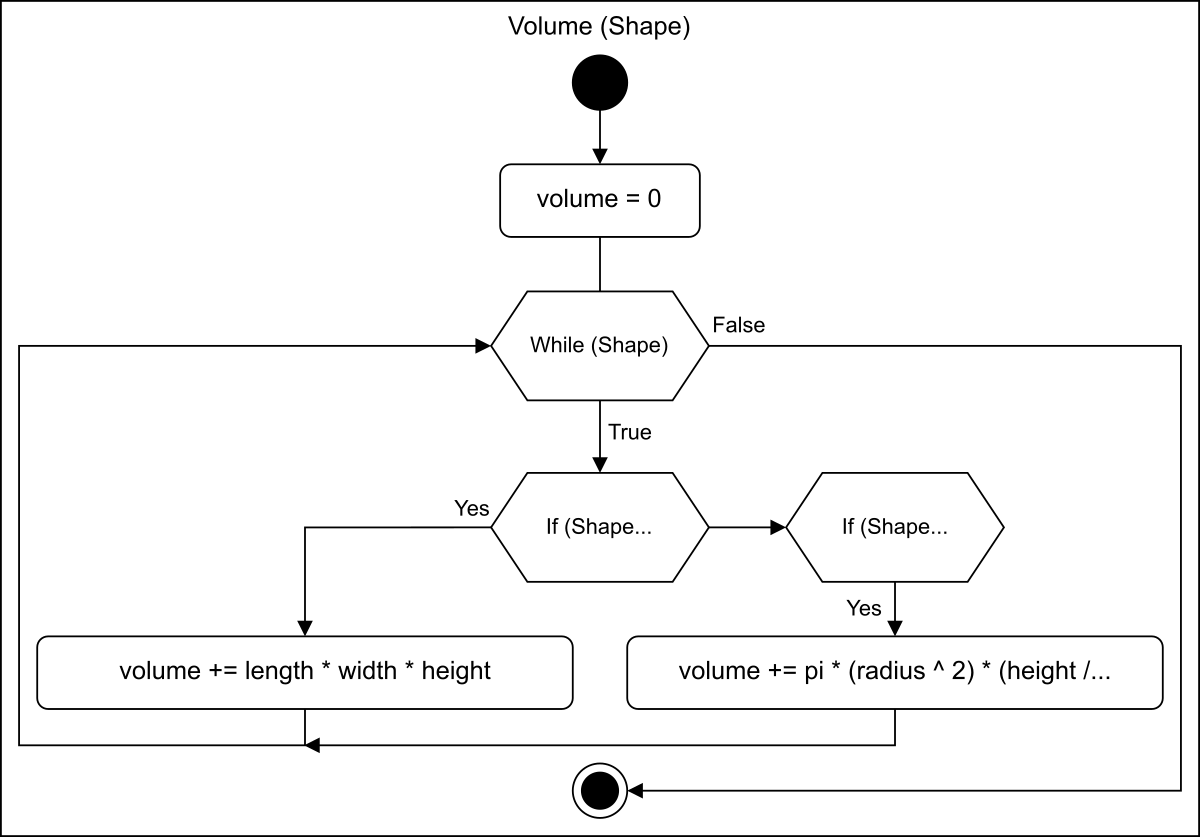
\includegraphics[width=0.5\textwidth]{Images/chapter_4/section_6348852334690304/4577764419305472.png}
 \caption{The volume (Shape) function}
\end{figure}

With only two types of boxes, the class structure looks fine, but what if Alex decides to deal with more types of boxes, e.g., a cylinder box? This will add complexity to the \texttt{volume(Shape)}. We will divide the code into segments using OCP to overcome this complexity.

\subsubsection{Implementing the Open Closed Principle}\label{hFd7rpt08wXBeLTsSs1hK}
\\
We will make a parent class, \texttt{Shape}, which is an abstract class and has a \texttt{volume()} function, that is extended by its sub-classes, \texttt{Cuboid}, \texttt{Cylinder}, and \texttt{Cone}. These derived classes have their own \texttt{volume()} functions according to the shape. Then we have the \texttt{VolumeCalculator} class that only performs one task: adding the volume of all the boxes using the \texttt{sumVolume()} function.

\begin{figure}[htbp]
 \centering
 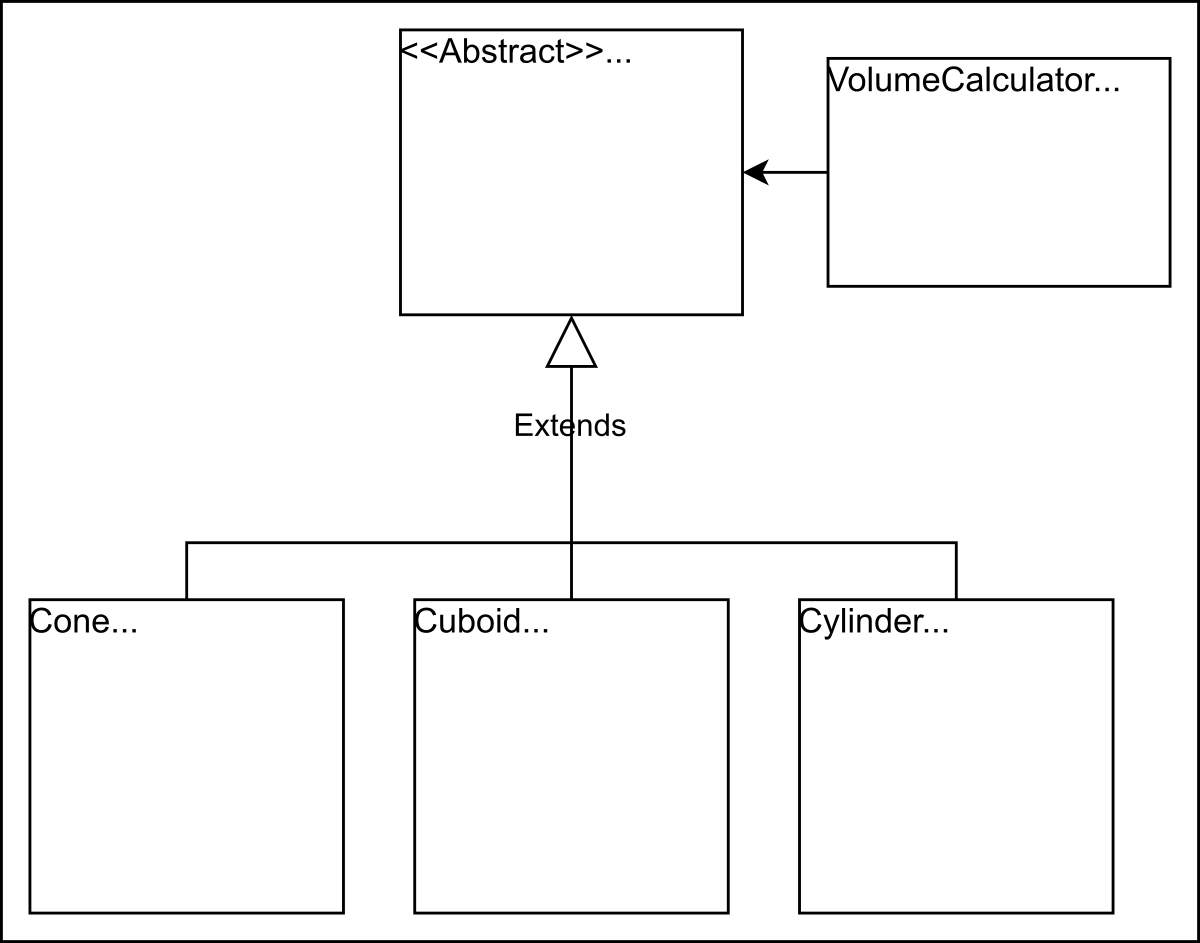
\includegraphics[width=0.5\textwidth]{Images/chapter_4/section_6348852334690304/5928312779833344.png}
 \caption{The class diagram of VolumeCalculator according to OCP}
\end{figure}

\subsection{Conclusion}\label{xejmKGo3pFfPq2z_eQZby}
\\
We can conclude the OCP discussion as follows:

\begin{itemize}
\item
\protect\phantomsection\label{Sfkvh9NJtgdZ1jlZgBmyO}
A software system should be easy to extend without the need for modification in the existing system. For the software systems, this goal is achieved by OCP.
\item
\protect\phantomsection\label{EXiw0J2JR5LOqEEm8fb2K}
The system must be divided into small components, which are arranged, so that core code is always protected from new code.
\end{itemize}
\\
In the next lesson, we will talk about the Liskov Substitution Principle with its detailed explanation.

% End of section content